\subsection*{\textit{\textbf{RQ6: What are the most influential attributes for identifying the
issues that will suffer from a long delivery delay?}}}

\begin{figure}
	\centering
	\subfloat[Eclipse]{
		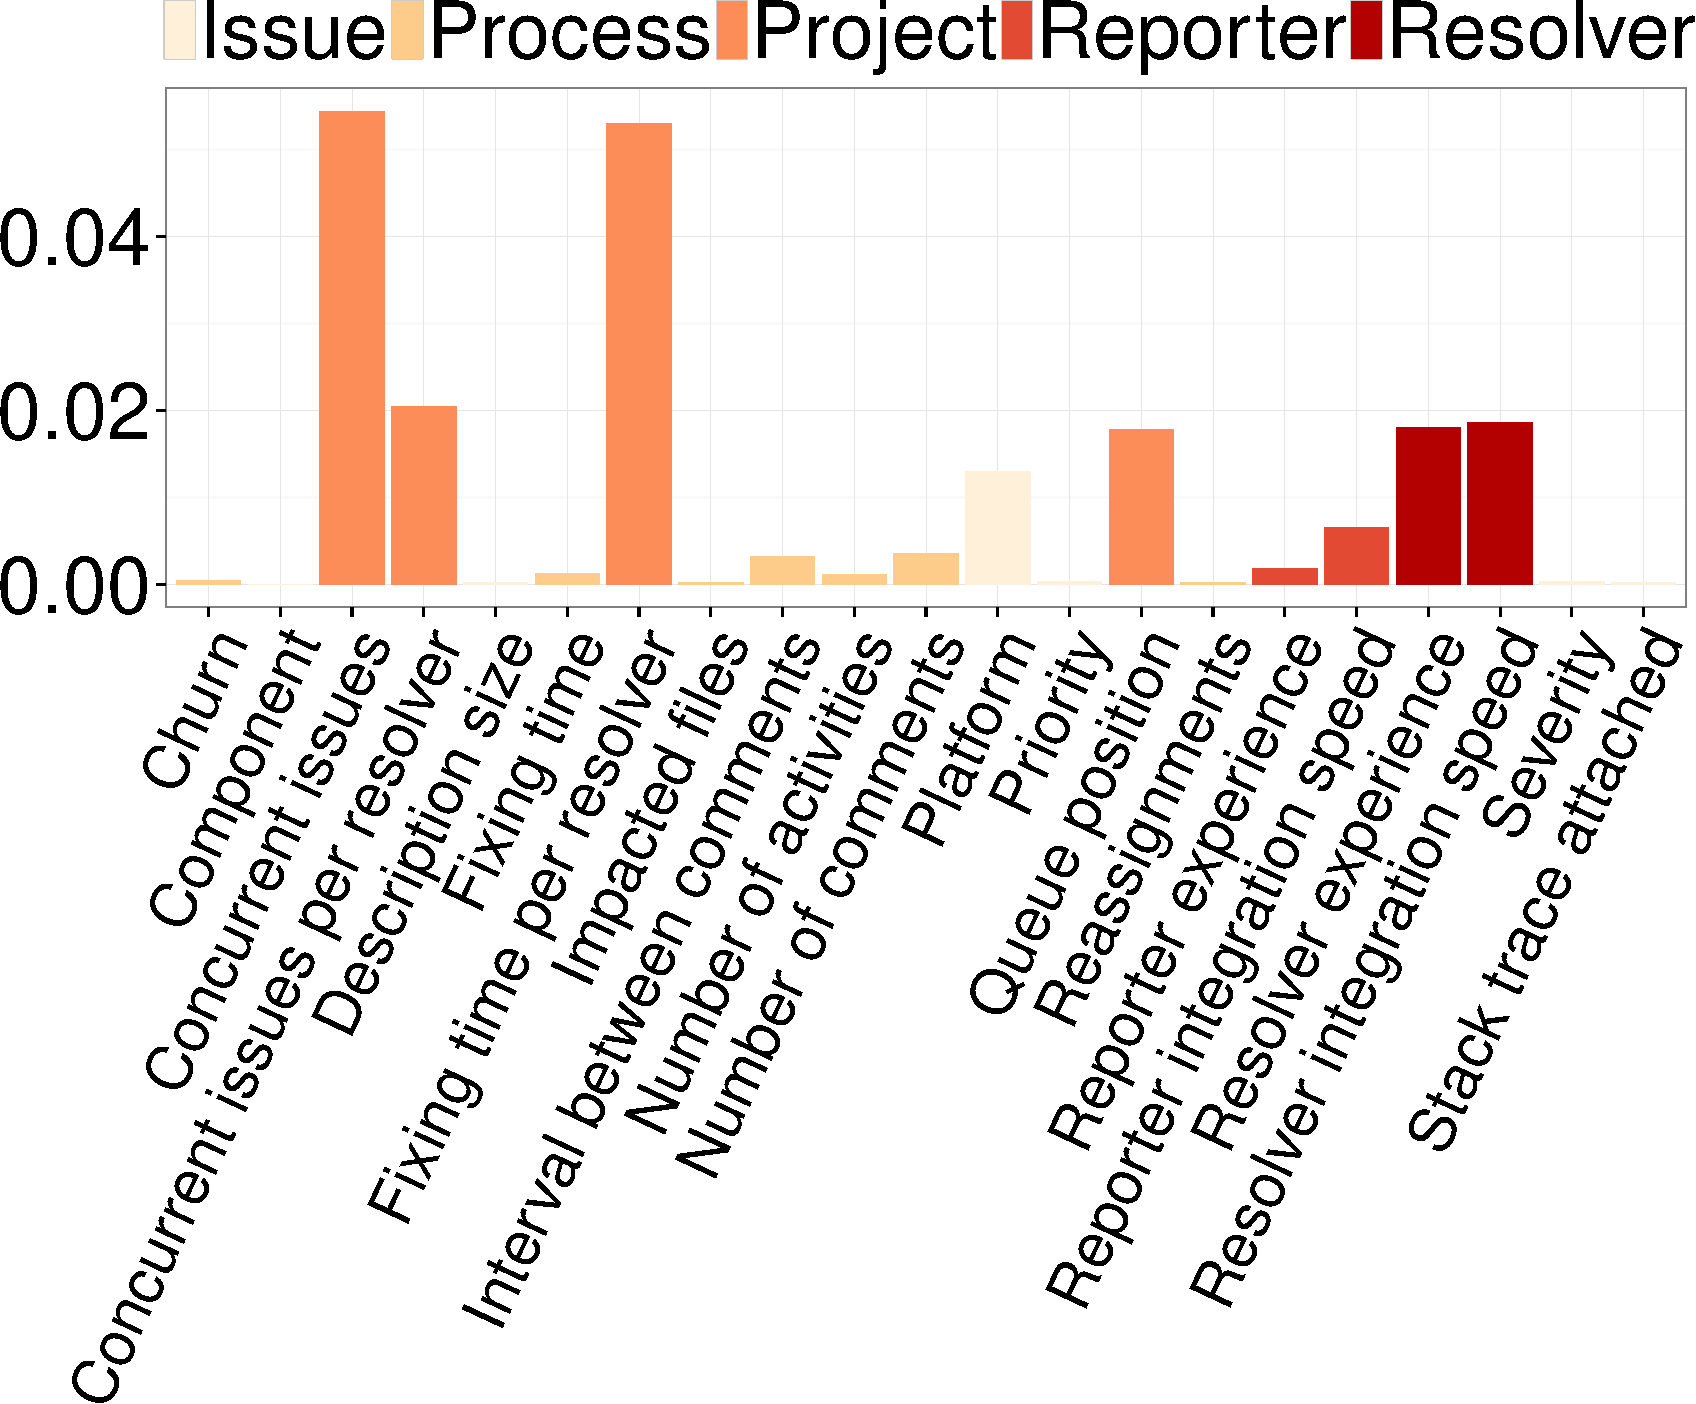
\includegraphics[width=0.50\textwidth,keepaspectratio] 
		{chapters/chapter4/figures/eclipse_loocv_varimp_long.pdf}
	\label{ch4:fig:impEclipse_ab}}

	\subfloat[Firefox]{
		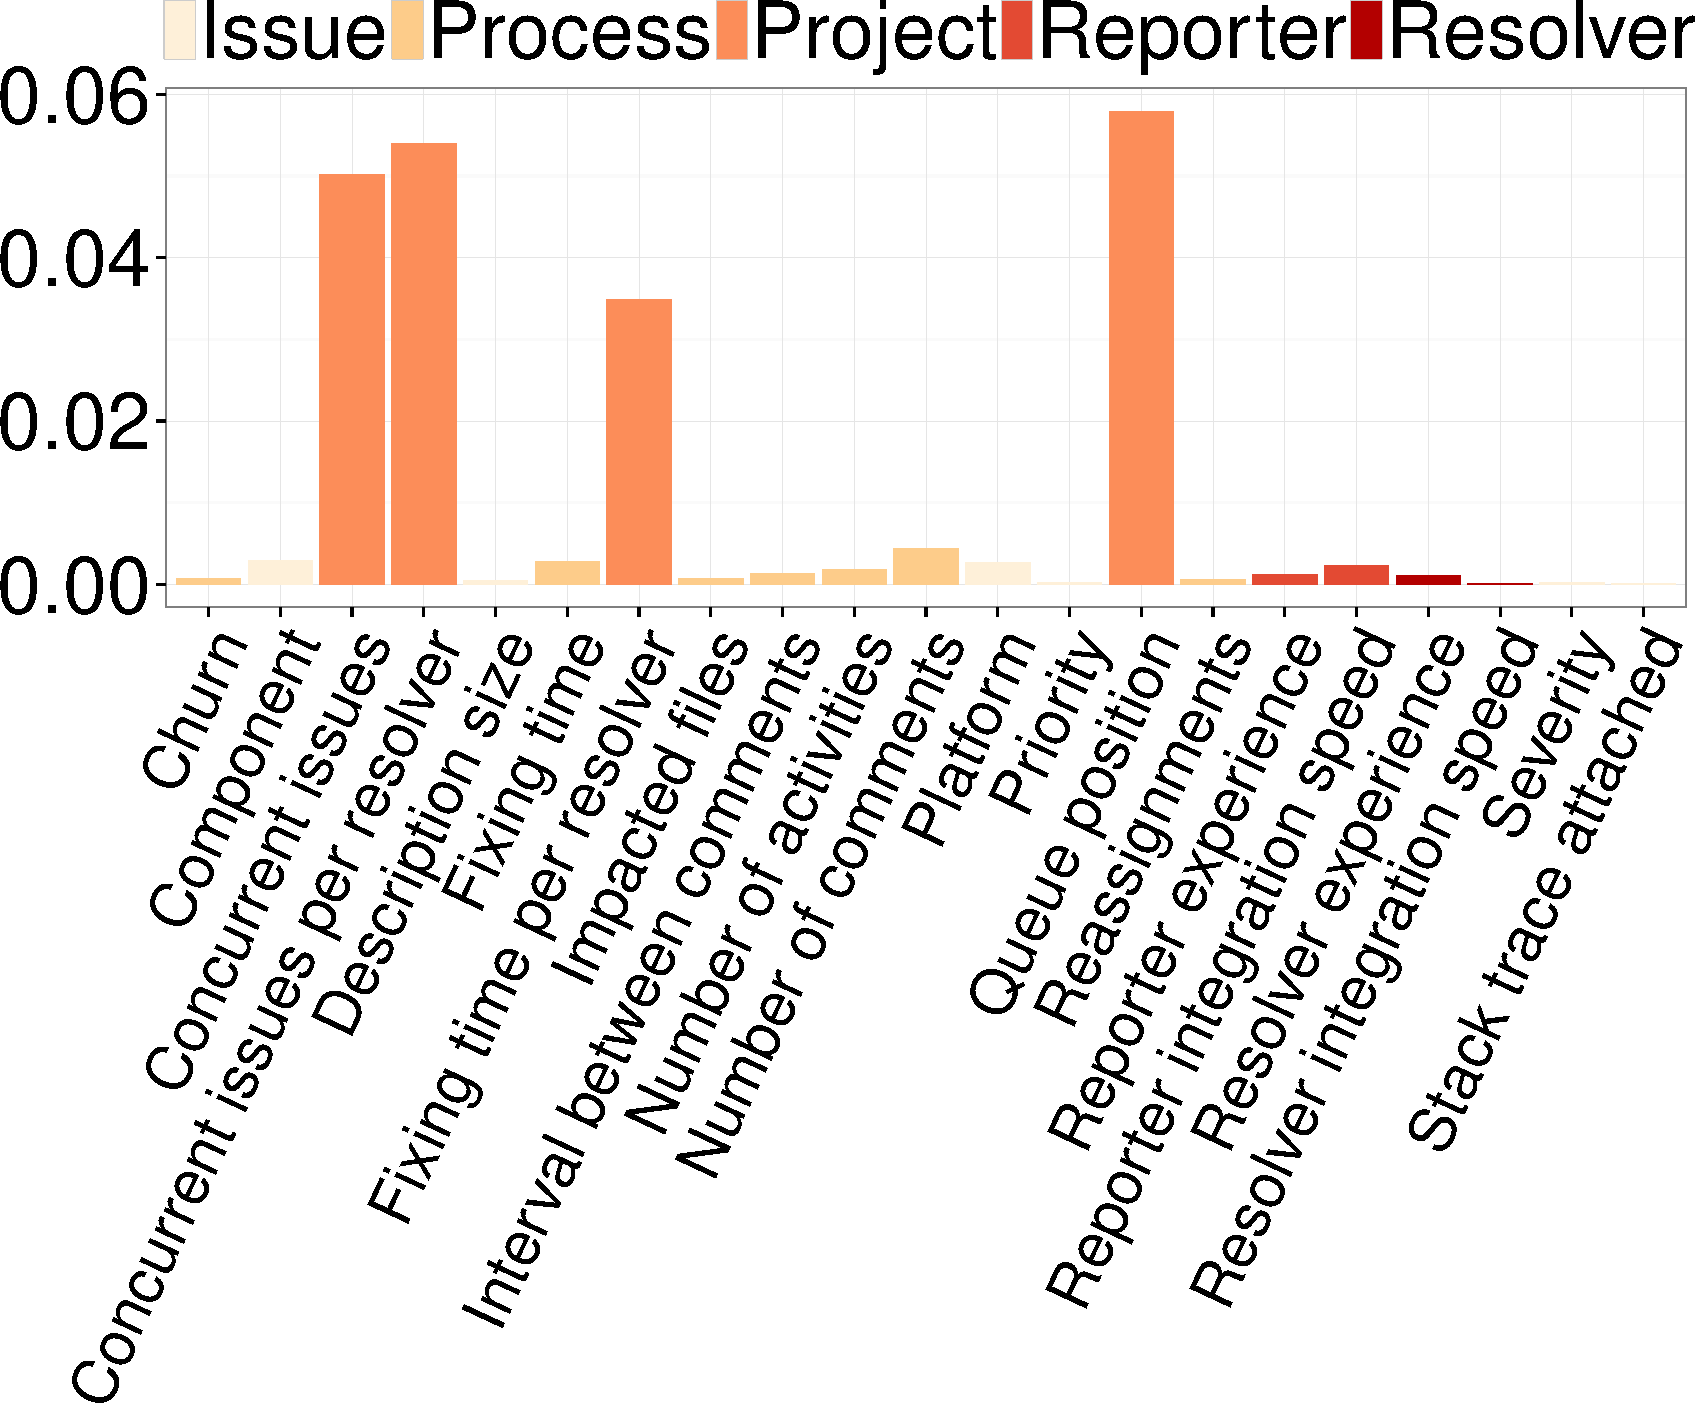
\includegraphics[width=0.50\textwidth,keepaspectratio]  
		{chapters/chapter4/figures/firefox_loocv_varimp_long.pdf}
		\label{ch4:fig:impFirefox_ab}
	}

	\subfloat[ArgoUML]{
		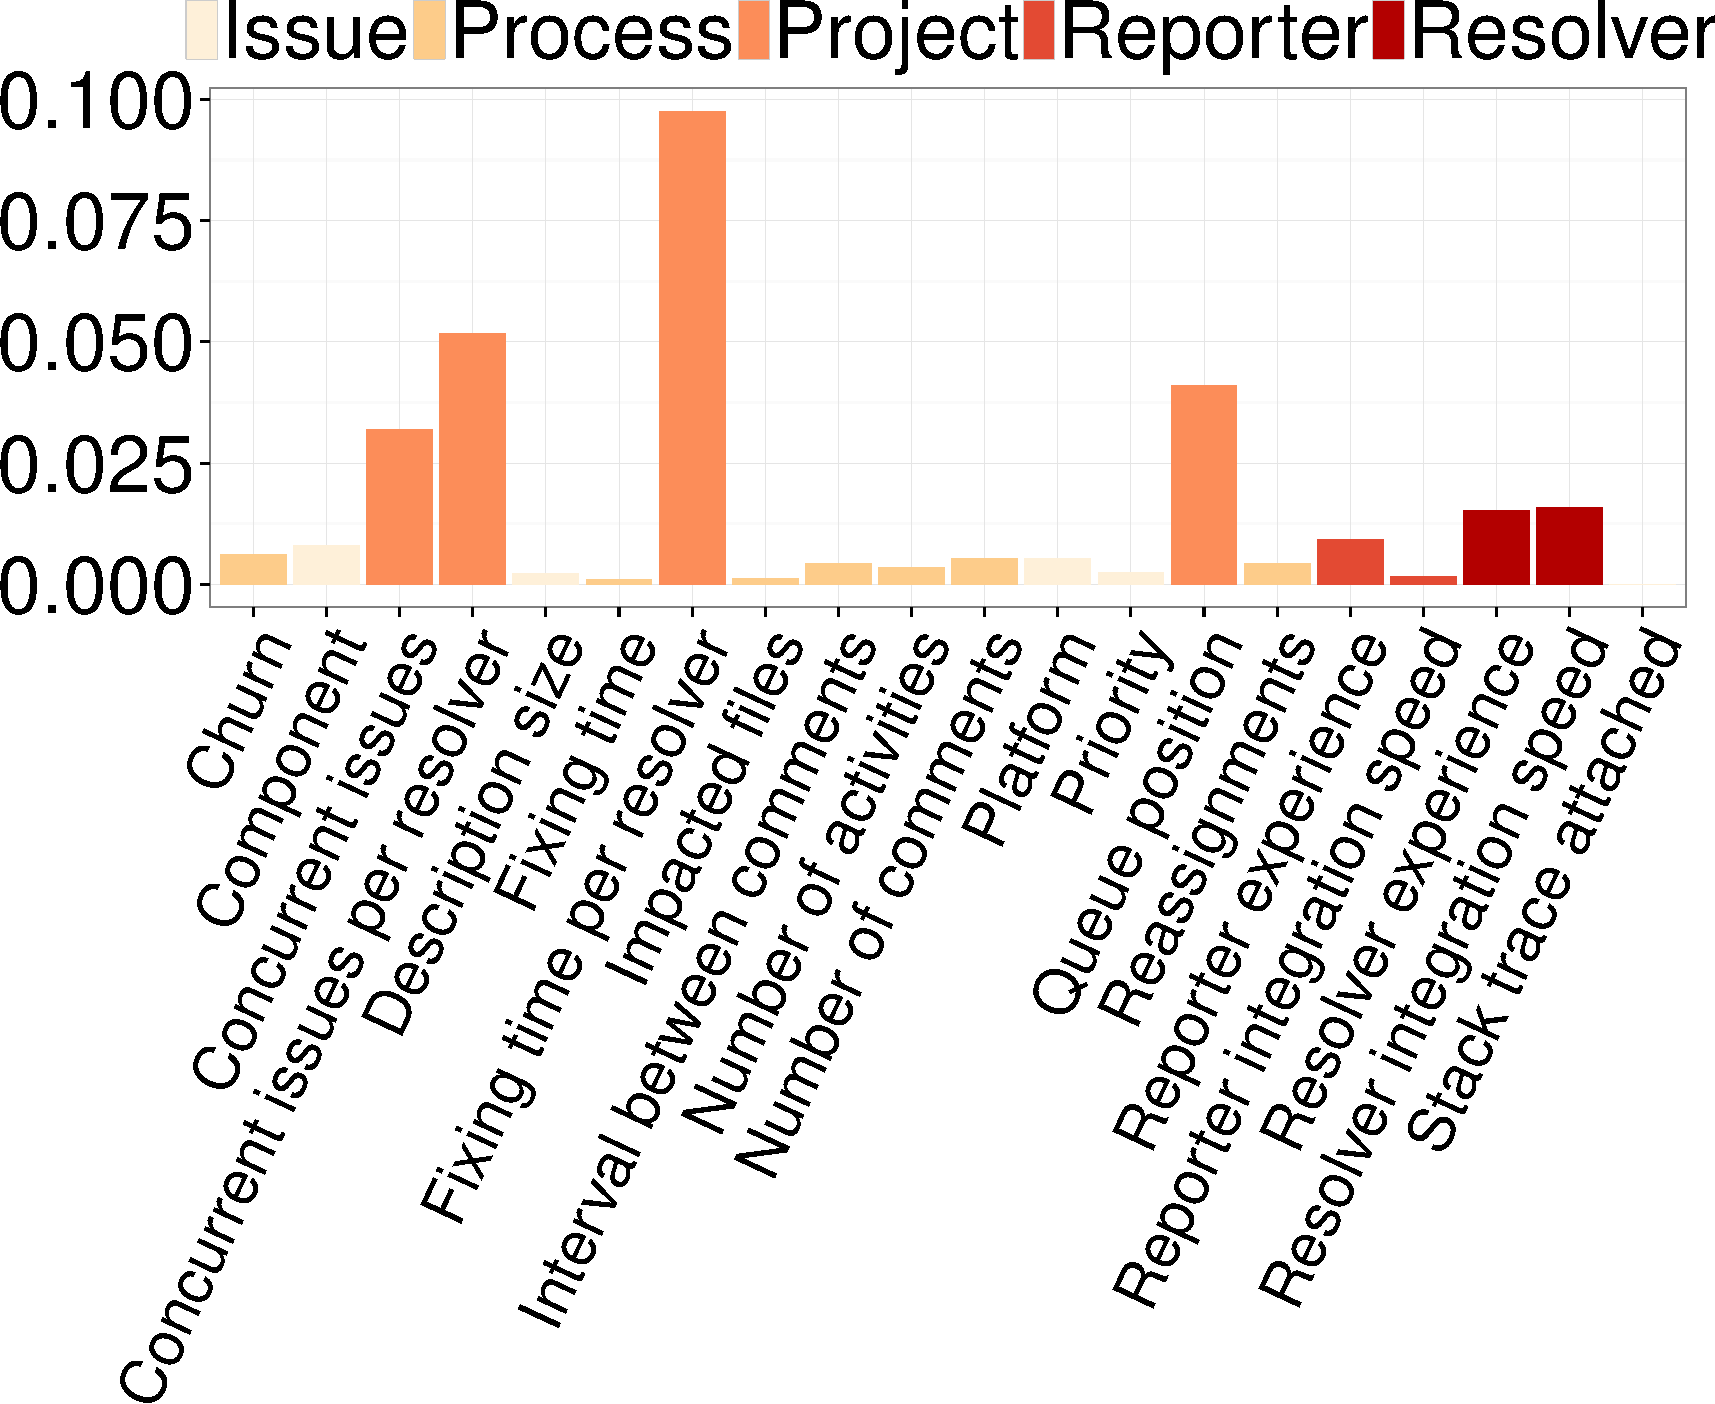
\includegraphics[width=0.50\textwidth,keepaspectratio] 
		{chapters/chapter4/figures/argouml_loocv_varimp_long.pdf}
	\label{ch4:fig:impArgo}}
	\caption{\textbf{Variable importance scores.} We show the 
	importance scores that are computed for the LOOCV of our models.}
	\label{ch4:fig:variableImportance_ab}
\end{figure}


\noindent\textit{\textbf{Long delivery delay is most consistently associated with
attributes of the project family.}}
\hyperref[ch4:fig:variableImportance_ab]{Figure}~\ref{ch4:fig:variableImportance_ab}
shows the importance scores that are computed for the LOOCV that we use to
evaluate our random forest models. We observe that the attributes that are
related to the \textit{\textbf{project}} family are the most influential
attributes in the projects. The \textit{backlog of issues} is the most
influential attribute in our Eclipse models, while \textit{queue position} and
\textit{fixing time per resolver} are the most influential attributes in our
Firefox and ArgoUML models, respectively. In addition, we observe that
attributes that are related to workload, such as the \textit{backlog of issues}
and the \textit{backlog of issues per resolver} are at least the third most
influential attributes in all of our models. Such results suggest that a
\textit{long delivery delay} is associated with project-related attributes and
that the amount of addressed issues that are to be integrated also plays a major
role to identify a \textit{long delivery delay}. \\

\conclusionbox{Our explanatory models suggest that long delivery delay is more
	closely associated with project characteristics, such as
	the \textit{backlog of issues}, \textit{queue position}, and
	\textit{fixing time per resolver}. Moreover, the backlog of issues plays an
	influential role in identifying a long delivery delay in all of the studied
projects.}

\section{Discussion}\label{ch4:discussion}

\noindent\textbf{\textit{The most important attributes vary as we study
different kinds of delivery delay.}} While we observe that \textit{fixing time
per resolver} is the most influential attribute to model delivery delay in
terms of releases, the time at which an issue is addressed (\textit{queue position})
is the most influential attribute to model delivery delay in days.  This
difference may be explained by what these kinds of delivery delay highlight.
The delivery delay in terms of releases highlights the releases from which the
integration of addressed issues is prevented. In this context, the \textit{fixing
time per resolver} attribute becomes influential, since it is a measure of the
amount of time that was invested by the team to fix issues, which may lead to
smoother integration of an issue in the upcoming releases. This smoother
integration might be either because issues were addressed more carefully or because
complex/risky issues had the necessary time to become stable enough to avoid
breakage. 

On the other hand, delivery delay in terms of days highlights the total time
that is required to ship an addressed issue regardless the number of releases that
are missed. In this case, the time at which an issue is addressed in the release
cycle becomes more influential (\ie \textit{queue position}). For example, a
addressed issue might be shipped faster because it was addressed during a {\em beta
stage} (see \hyperref{ch4:rq2}{RQ2}), \ie when the collaborators have to deal with a
narrower \textit{backlog of issues} so that fixes can be performed more
carefully. The increased focus due to a narrower \textit{backlog of issues} may
lead the addressed issue to become easier to integrate in the next release cycle.

Moreover, in the Eclipse project, we observe that the speed at which the prior
addressed issues of a particular resolver are integrated influences the integration
time of new addressed issues (\textit{resolver integration speed}). This result
might be an indicator that resolvers/integrators who are experienced
in fixing and integrating fixes for the project may reduce delivery delay.

As for long delivery delay, we observe a similar behaviour in our models that
are fit to the ArgoUML and Eclipse projects. The \textit{fixing time per
resolver} attribute and attributes that are related to the \textit{backlog of
issues} are the most important to identify addressed issues that have a long
delivery delay. On the other hand, the \textit{queue position} is the most
important attribute to model long delivery delay in the Firefox project. One of
the major differences between the former projects (ArgoUML and Eclipse) and the
later one (Firefox) is the release cycle strategy that is adopted---ArgoUML and
Eclipse use a more traditional release cycle compared to the rapid release
cycles that are used in the Firefox project. Nevertheless, more empirical
analyses are necessary to investigate if there is a relationship between release
cycle strategies and prolonged delivery delay.\\

\noindent\textbf{\textit{The backlog of addressed issues awaiting integration
may introduce an overhead that needs to be managed by software teams.}} We
observe that integration workload attributes (\eg \textit{backlog of issues} and
\textit{backlog of issues per resolver}) are influential in all studied kinds of
delivery delay. This finding suggests that the overhead that is introduced by
the backlog of addressed issues that are awaiting integration may increase the
integration time as a whole. 

